% !TeX program = lualatex
\documentclass[aspectratio=169,12pt]{beamer}

% ------------------------------------------------------------
% Fonts and language
% ------------------------------------------------------------
\usepackage{fontspec}
\setsansfont{Arial}[Ligatures=TeX]
\setmainfont{Arial}[Ligatures=TeX]
\setmonofont{Courier New}[Scale=0.9, Ligatures=TeX]

\newfontfamily\cyrillicfont{Arial}[Script=Cyrillic, Ligatures=TeX]
\newfontfamily\cyrillicfontsf{Arial}[Script=Cyrillic, Ligatures=TeX]
\newfontfamily\cyrillicfonttt{Courier New}[Scale=0.9, Script=Cyrillic, Ligatures=TeX]

\usepackage{polyglossia}
\setdefaultlanguage{russian}
\setotherlanguage{english}

% ------------------------------------------------------------
% Packages
% ------------------------------------------------------------
\usepackage{amsmath,amssymb,mathtools}
\usepackage{graphicx}
\usepackage{xcolor}
\usepackage{tikz}
\usetikzlibrary{arrows.meta,positioning}

% Пути: работает при компиляции из папки presentation
\graphicspath{
  {images/}
  {../images/}
  {../images_appendix/}
  {../figures/}
}

% ------------------------------------------------------------
% Style
% ------------------------------------------------------------
\definecolor{rudnblue}{HTML}{0070C0}
\definecolor{rudndarkblue}{HTML}{005B9E}
\definecolor{rudngreen}{HTML}{00843D}
\definecolor{rudnred}{HTML}{C8102E}
\definecolor{lightblue}{HTML}{EAF4FB}

\usetheme{default}
\usefonttheme{professionalfonts}
\setbeamertemplate{navigation symbols}{}
\setbeamersize{text margin left=0.65cm, text margin right=0.65cm}

\setbeamercolor{background canvas}{bg=white}
\setbeamercolor{normal text}{fg=black}
\setbeamercolor{frametitle}{fg=rudnblue,bg=white}
\setbeamerfont{frametitle}{size=\LARGE,series=\bfseries}
\setbeamerfont{normal text}{size=\large}

\setbeamertemplate{itemize item}{\color{rudnblue}$\blacktriangleright$}
\setbeamertemplate{itemize subitem}{\color{rudnblue}$\bullet$}

\setbeamertemplate{frametitle}{
  \vspace{0.35cm}
  \insertframetitle
  \vspace{0.10cm}
}

% Нижняя линия + номер + логотип РУДН
\setbeamertemplate{footline}{
  \begin{tikzpicture}[remember picture,overlay]

    % красно-зелёная линия
    \draw[rudnred, line width=1.1pt]
      ([xshift=0.45cm,yshift=0.47cm]current page.south west)
      -- ([xshift=-3.55cm,yshift=0.47cm]current page.south east);

    \draw[rudngreen, line width=1.6pt]
      ([xshift=0.45cm,yshift=0.34cm]current page.south west)
      -- ([xshift=-3.55cm,yshift=0.34cm]current page.south east);

    % номер поверх линии, с белым фоном
    \node[
      anchor=south west,
      fill=white,
      inner xsep=2pt,
      inner ysep=1pt,
      text=rudnblue,
      font=\bfseries\small
    ] at ([xshift=0.15cm,yshift=0.25cm]current page.south west)
      {\insertframenumber/\inserttotalframenumber};

    % логотип справа
    \node[
      anchor=south east,
      inner sep=0pt
    ] at ([xshift=-0.25cm,yshift=0.13cm]current page.south east)
      {
\includegraphics[width=2.75cm]{rudn_blue.png}};

  \end{tikzpicture}
  \vspace{0.70cm}
}

\newcommand{\slideconclusion}[1]{
  \vspace{0.25cm}
  {\large\bfseries #1}
}

% ------------------------------------------------------------
% Document
% ------------------------------------------------------------
\begin{document}
% ------------------------------------------------------------
% 1. Титульный слайд из PDF как фон
% ------------------------------------------------------------
{
\setbeamertemplate{footline}{}
\usebackgroundtemplate{%
  \includegraphics[width=\paperwidth,height=\paperheight]{Титульник.pdf}%
}
\begin{frame}[plain]
\end{frame}
\usebackgroundtemplate{}
}
% ------------------------------------------------------------
% 2. Goal
% ------------------------------------------------------------
\begin{frame}{Цель и задачи работы}

\textbf{Цель:} исследовать чувствительность стационарных характеристик
ресурсной СМО с потерями $GI/G/N/N/R$ к распределению времени обслуживания
и типу входящего потока.

\vspace{0.45cm}

\textbf{Задачи:}
\begin{enumerate}
  \item сформулировать модель РСМО с потерями, ограниченными каналами и ресурсами;
  \item определить набор исследуемых стационарных характеристик;
  \item задать распределения входящего потока и объёма работы заявки;
  \item разработать алгоритм имитационного моделирования;
  \item реализовать программно-вычислительный комплекс;
  \item провести вычислительные эксперименты и проанализировать влияние параметров на характеристики системы;
\end{enumerate}

\end{frame}

% ------------------------------------------------------------
% 3. Формальная постановка
% ------------------------------------------------------------
\begin{frame}{Формальная постановка модели}

Сценарий задаётся набором параметров:
$$
s = (a,\omega,\lambda,\mu,N,R,F_D),
$$

\vspace{-0.2cm}

\begin{itemize}
  \item $a$ — распределение входящего потока;
  \item $\omega$ — распределение объёма работы заявки;
  \item $\lambda$ — средняя интенсивность поступления;
  \item $\mu$ — скорость обслуживания на прибор;
  \item $N$ — число обслуживающих приборов;
  \item $R$ — общий объём ресурса;
  \item $F_D$ — распределение ресурсного требования.
\end{itemize}

\end{frame}

% ------------------------------------------------------------
% 4. Механизм потерь
% ------------------------------------------------------------
\begin{frame}{Механизм потерь в системе $GI/G/N/N/R$}

Время задается дискретно-событийно, в каждый момент $t$ имеется $n(t)$ — число заявок в системе и $u(t)$ — занятый ресурс.

Входящая заявка имеет требование к ресурсу $D_i$. 

\vspace{0.3cm}

Новая заявка принимается, если выполнены оба условия:
$$
\begin{cases}
n(t_i-) < N,\\
u(t_i-) + D_i \leq R.
\end{cases}
$$

%\vspace{0.3cm}

Если хотя бы одно условие нарушено, заявка теряется.

\end{frame}

% ------------------------------------------------------------
% 4.1. Семейства распределений в РСМО
% ------------------------------------------------------------
\begin{frame}{Семейства распределений в модели}

% В исследуемой системе $GI/G/N/N/R$ одновременно варьируются вероятностные механизмы прихода заявок и их обработки.

%\vspace{0.2cm}

%\textbf{Ключевые принципы построения экспериментов:}
\begin{itemize}
  \item \textbf{Нормировка по первому моменту} для отделения влияния дисперсии от уровня средней нагрузки. Математические ожидания строго фиксированы:
  $$ \mathbb{E}[A] = \frac{1}{\lambda}, \qquad \mathbb{E}[W] = 1, \qquad \mathbb{E}[S] = \frac{1}{\mu} $$
  \item \textbf{Интенсивность входящего потока и времени работы заявки} отличаются формой распределений, которая характеризуется квадратом коэффициента вариации:
  $$ c_A^2 = \frac{\operatorname{Var}(A)}{\mathbb{E}[A]^2}, \qquad c_W^2 = \frac{\operatorname{Var}(W)}{\mathbb{E}[W]^2} $$
\end{itemize}



\end{frame}

% ------------------------------------------------------------
% 4.2. Моделирование входящего потока
% ------------------------------------------------------------
\begin{frame}{Моделирование входящего потока}

В зависимости от значения $c_A^2$ формируются сценарии нагрузки разной степени регулярности.

\vspace{0.2cm}
\begin{center}
\small
\renewcommand{\arraystretch}{1.3}
\begin{tabular}{l|c|c|l}
  \textbf{Входящий поток} & \textbf{Распределение} & $c_A^2$ & \textbf{Режим нагрузки} \\ \hline
  \color{rudnblue}\textbf{Пуассоновский} & $\operatorname{Exp}(\lambda)$ & $1.0$ & Базовый ($M/G/N/N/R$) \\
  \textbf{Эрланга (k=2)} & $\operatorname{Erlang}(2, 2\lambda)$ & $0.5$ & Регулярный \\
  \textbf{Эрланга (k=4)} & $\operatorname{Erlang}(4, 4\lambda)$ & $0.25$ & Высокорегулярный \\
  \textbf{Гиперэкспон.} & Смесь $H_2$ & $> 1.0$ & Пачечный (всплески) \\
\end{tabular}
\end{center}

\vspace{0.3cm}
\flushleft
\slideconclusion{Базовый сценарий -- Пуассоновский входящий поток.}

\end{frame}

% ------------------------------------------------------------
% 4.3. Моделирование объема работы заявки
% ------------------------------------------------------------
\begin{frame}{Моделирование объема работы заявки}

Варьирование распределения объема работы $W$ (при $\mathbb{E}[W]=1$) определяет разброс времени обслуживания задач на приборах.

\vspace{0.2cm}
\begin{center}
\small
\renewcommand{\arraystretch}{1.3}
\begin{tabular}{l|c|c|l}
  \textbf{Обслуживание} & \textbf{Распределение} & $c_W^2$ & \textbf{Характер задач} \\ \hline
  \color{rudnblue}\textbf{Детерминиров.} & $W \equiv 1$ & $0.0$ & Полная предсказуемость \\
  \textbf{Эрланга (k=4)} & $\operatorname{Erlang}(4, 4)$ & $0.25$ & Устойчивое время \\
  \textbf{Экспоненциал.} & $\operatorname{Exp}(1)$ & $1.0$ & Марковский базис \\
  \textbf{Гиперэкспон.} & Смесь $H_{\mathrm{heavy}}$ & $> 1.0$ & Короткие + тяжелые \\
\end{tabular}
\end{center}

\vspace{0.3cm}
\flushleft
\slideconclusion{Базовый сценарий -- Детерминированное время работы.}

\end{frame}
% ------------------------------------------------------------
% 5а. Оцениваемые показатели: потоковые метрики
% ------------------------------------------------------------
\begin{frame}{Оцениваемые потоковые метрики}

Сбор статистических данных ведется после периода разогрева:
$T_{\mathrm{obs}} = T_{\max} - T_{\mathrm{warm}}$.

\vspace{0.4cm}

\textbf{Вероятность отказа (блокировки заявок)} определяется как доля отклоненных задач среди всех поступивших за время наблюдения:
\[
\widehat{P}_{\mathrm{loss}} = \frac{N_{\mathrm{rej}}}{N_{\mathrm{arr}}}
\]

%\vspace{0.3cm}

\textbf{Абсолютная пропускная способность}  определяется как среднее число принятых заявок в единицу модельного времени:
\[
\widehat{\theta} = \frac{N_{\mathrm{acc}}}{T_{\mathrm{obs}}}
\]

%\vspace{0.3cm}
Также отслеживается среднее время обслуживания $\widehat{\mathbb{E}}[S]$ и время пребывания заявки в системе $\widehat{\mathbb{E}}[T_{\mathrm{soj}}]$.

\end{frame}

% ------------------------------------------------------------
% 5б. Оцениваемые показатели: временные средние
% ------------------------------------------------------------
\begin{frame}{Оцениваемые временные средние}

Поскольку логика работы симулятора является дискретно-событийной, непрерывные интегралы во времени рассчитываются как суммы площадей по межсобытийным интервалам $\Delta t_j$:

\vspace{0.3cm}

\textbf{Среднее число заявок в системе:}
\[
\widehat{\mathbb{E}}[n] = \frac{1}{T_{\mathrm{obs}}} \int_{T_{\mathrm{warm}}}^{T_{\max}} n(t)\,dt = \frac{1}{T_{\mathrm{obs}}} \sum_{j} n_j \Delta t_j
\]

\vspace{0.4cm}

\textbf{Математическое ожидание занятого ресурса:}
\[
\widehat{\mathbb{E}}[u] = \frac{1}{T_{\mathrm{obs}}} \int_{T_{\mathrm{warm}}}^{T_{\max}} u(t)\,dt = \frac{1}{T_{\mathrm{obs}}} \sum_{j} u_{j} \Delta t_j
\]

\end{frame}
% ------------------------------------------------------------
% 6. Сетка сценариев эксперимента
% ------------------------------------------------------------
\begin{frame}{Сетка сценариев эксперимента}

Сценарий $s$ — это точка в пространстве параметров. Для комп. имитации крайне важны множества:
$A$ — типы входящего потока, $\Omega$ — распределения времени работы, 
$\Lambda$ — уровни интенсивности поступления, $\mathrm{M}$ — скорость обслуживания.

\vspace{0.2cm}
\textbf{Дизайн экспериментов (декартовы произведения определяют его сложность):}
\begin{itemize}
    \item \text{Базовый:} \quad $\Lambda \times \mathrm{M}$
    \item \text{Чувствительность к workload:} \quad $\Omega \times \Lambda \times \mathrm{M}$
    \item \text{Чувствительность к arrival:} \quad $A \times \Lambda \times \mathrm{M}$
    \item \text{Совместное влияние:} \quad $\Omega \times A \times \Lambda \times \mathrm{M}$
\end{itemize}

\end{frame}

% ------------------------------------------------------------
% 6.1 Параметры системы
% ------------------------------------------------------------
\begin{frame}{Параметры моделируемой системы}

\textbf{1. Базовая архитектура и нагрузка:}
\begin{itemize}
    \item $N = 96$ серверов, суммарный доступный ресурс $R = 590$.
    \item Интенсивность $\lambda \in \{90, 104, 116\}$ (от недогрузки до перегрузки), $\mu = 1.2$.
\end{itemize}

\vspace{0.2cm}
\textbf{2. Формирование дефицита ресурса (узкого места):}
\begin{itemize}
    \item Требование $D \in \{2, 4, 8, 12, 16\}$ задано дискретно, $\mathbb{E}[D] = 6.5$.
    \item Потребность при полной занятости приборов: $N \cdot \mathbb{E}[D] = 624 > 590 \ (R)$.
    \item \textit{Следствие:} Главной причиной потерь становится нехватка ресурса $R$, что характерно для реальных сетей связи.
\end{itemize}

\vspace{0.2cm}
\textbf{3. Достоверность результатов (метод Монте-Карло):}
\begin{itemize}
    \item $T_{\max} = 50000$ (вкл. разогрев $T_{\mathrm{warm}} = 5000$).
    \item $R_{\mathrm{rep}} = 40$ независимых прогонов для получения 95\% доверительного интервала.
\end{itemize}

\end{frame}

% ------------------------------------------------------------
% 7. Вычислительная реализация
% ------------------------------------------------------------
\begin{frame}{Архитектура и вычислительная реализация}

Отсутствие зависимости от состояний позволяет применить массовое распараллеливание методом Монте-Карло:
\[ N_{\mathrm{runs}} = N_{\mathrm{scenarios}} \times R_{\mathrm{rep}} \quad \longrightarrow \quad \text{выполнение на ядрах GPU} \]

\vspace{0.2cm}
\begin{center}
\begin{tikzpicture}[
  block/.style={
    draw, rounded corners, align=center,
    minimum width=2.6cm, minimum height=1.0cm, font=\small, fill=lightblue
  },
  arrow/.style={-{Stealth[length=2.3mm]}, thick, rudndarkblue}
]
\node[block] (py1) {Python\\конфигурация};
\node[block, right=0.6cm of py1] (rust) {Rust\\оркестрация};
\node[block, right=0.6cm of rust] (cuda) {CUDA\\репликации};
\node[block, right=0.6cm of cuda] (py2) {Python\\агрегация и plots};

\draw[arrow] (py1) -- (rust);
\draw[arrow] (rust) -- (cuda);
\draw[arrow] (cuda) -- (py2);
\end{tikzpicture}
\end{center}

\vspace{0.2cm}
% Замени ссылку на свою реальную
%\slideconclusion{\href{https://github.com/PepsiMonster/Diplom}{\color{rudnblue}\textbf{GitHub:} https://github.com/PepsiMonster/Diplom}}

\end{frame}

% ------------------------------------------------------------
% 8.1. Workload: Инвариантность
% ------------------------------------------------------------
\begin{frame}{Инвариантность к обслуживанию}

\begin{columns}[T,totalwidth=\textwidth]
\begin{column}{0.45\textwidth}
\textbf{Условия эксперимента:}
\begin{itemize}
  \item Входящий поток: Пуассоновский (марковский базис).
  \item Фиксированное среднее время обслуживания $\mathbb{E}[S] = 1/\mu$.
  \item Варьируется только форма распределения $W$ (от константы до тяжелых хвостов).
\end{itemize}
\end{column}

\begin{column}{0.53\textwidth}
\centering
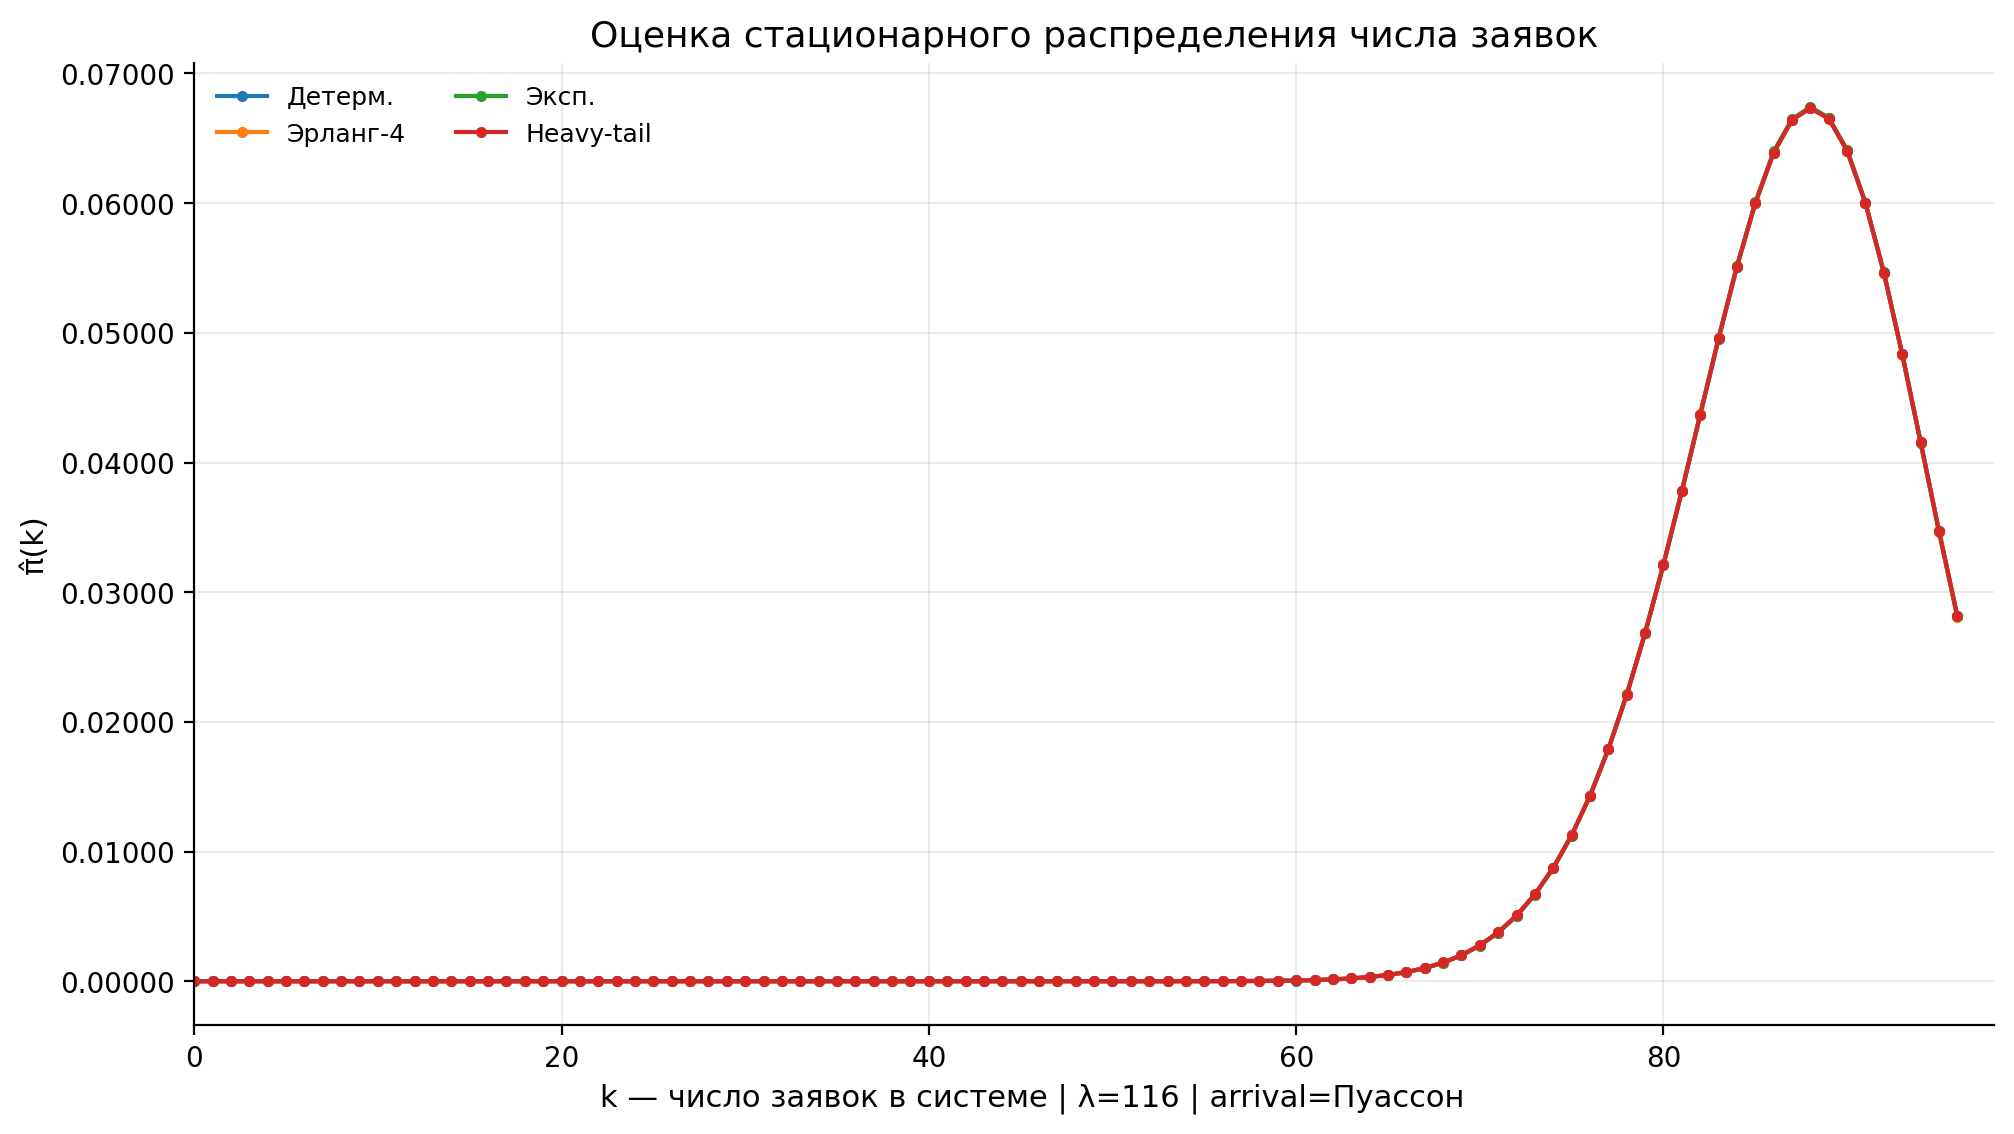
\includegraphics[
  width=\textwidth,
  height=0.55\textheight,
  keepaspectratio
]{workload_sensitivity_stationary_distribution_sigma-1p2_lambda-116.png}
\end{column}
\end{columns}

\vspace{0.1cm}
Кривые $\pi(k)$ сливаются. Свойство инвариантности макропоказателей в ресурсной модели $GI/G/N/N/R$ сохраняется.

\end{frame}

% ------------------------------------------------------------
% 8.2. Workload: Статистическое обоснование
% ------------------------------------------------------------
\begin{frame}{Статистическая верификация инвариантности}

\begin{columns}[T,totalwidth=\textwidth]
\begin{column}{0.45\textwidth}
\textbf{Анализ микроотклонений:}
\begin{itemize}
  \item Девиации вероятности отказа от марковского базиса составляют менее $0.02\%$.
  \item Межквартильные размахи независимых репликаций полностью перекрывают друг друга.
\end{itemize}
\end{column}

\begin{column}{0.53\textwidth}
\centering
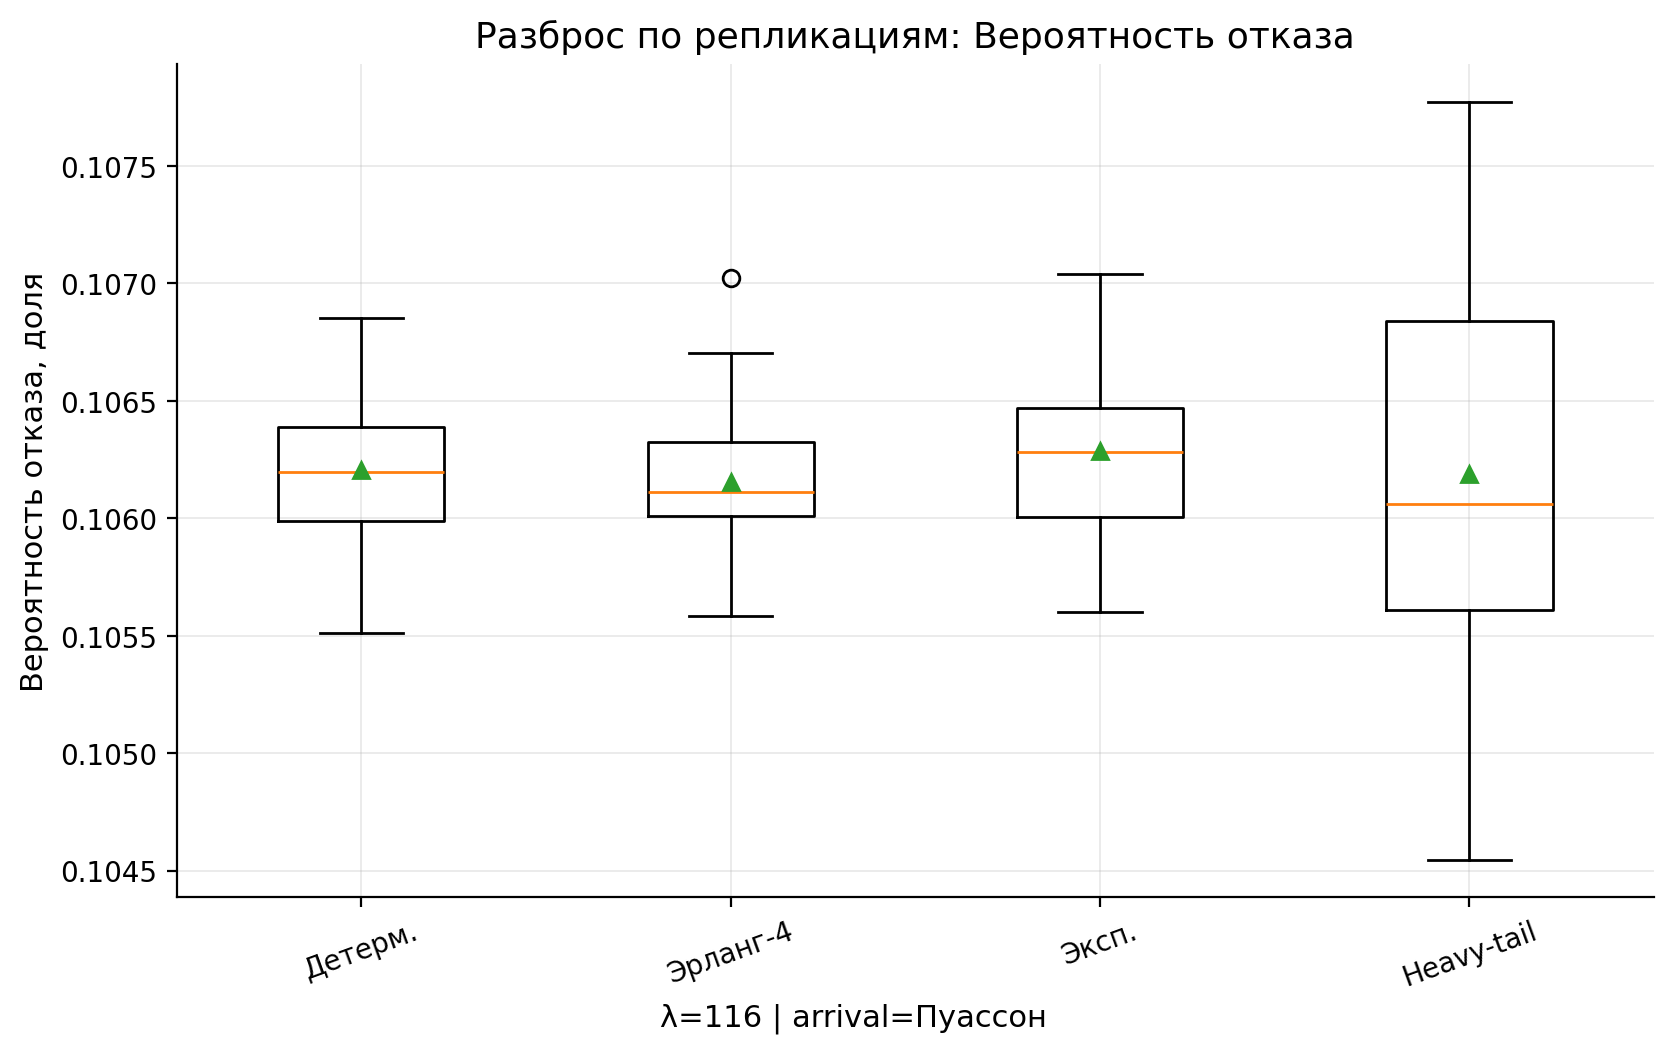
\includegraphics[
  width=\textwidth,
  height=0.55\textheight,
  keepaspectratio
]{workload_sensitivity_boxplot_loss_probability_sigma-1p2_lambda-116.png}
\end{column}
\end{columns}

\vspace{0.1cm}
Микрорасхождения объясняются шумом Монте-Карло. Допустимо использование аппроксимаций $M/M/N/R$ без потери точности.

\end{frame}
% ------------------------------------------------------------
% 9.1. Arrival: Главный фактор
% ------------------------------------------------------------
\begin{frame}{Чувствительность к типу входящего потока}

\begin{columns}[T,totalwidth=\textwidth]
\begin{column}{0.45\textwidth}
\textbf{Условия эксперимента:}
\begin{itemize}
  \item Фиксированное обслуживание: Детерминированное.
  \item Варьируется входящий поток при неизменном среднем $\mathbb{E}[A] = 1/\lambda$.
\end{itemize}
\end{column}

\begin{column}{0.53\textwidth}
\centering
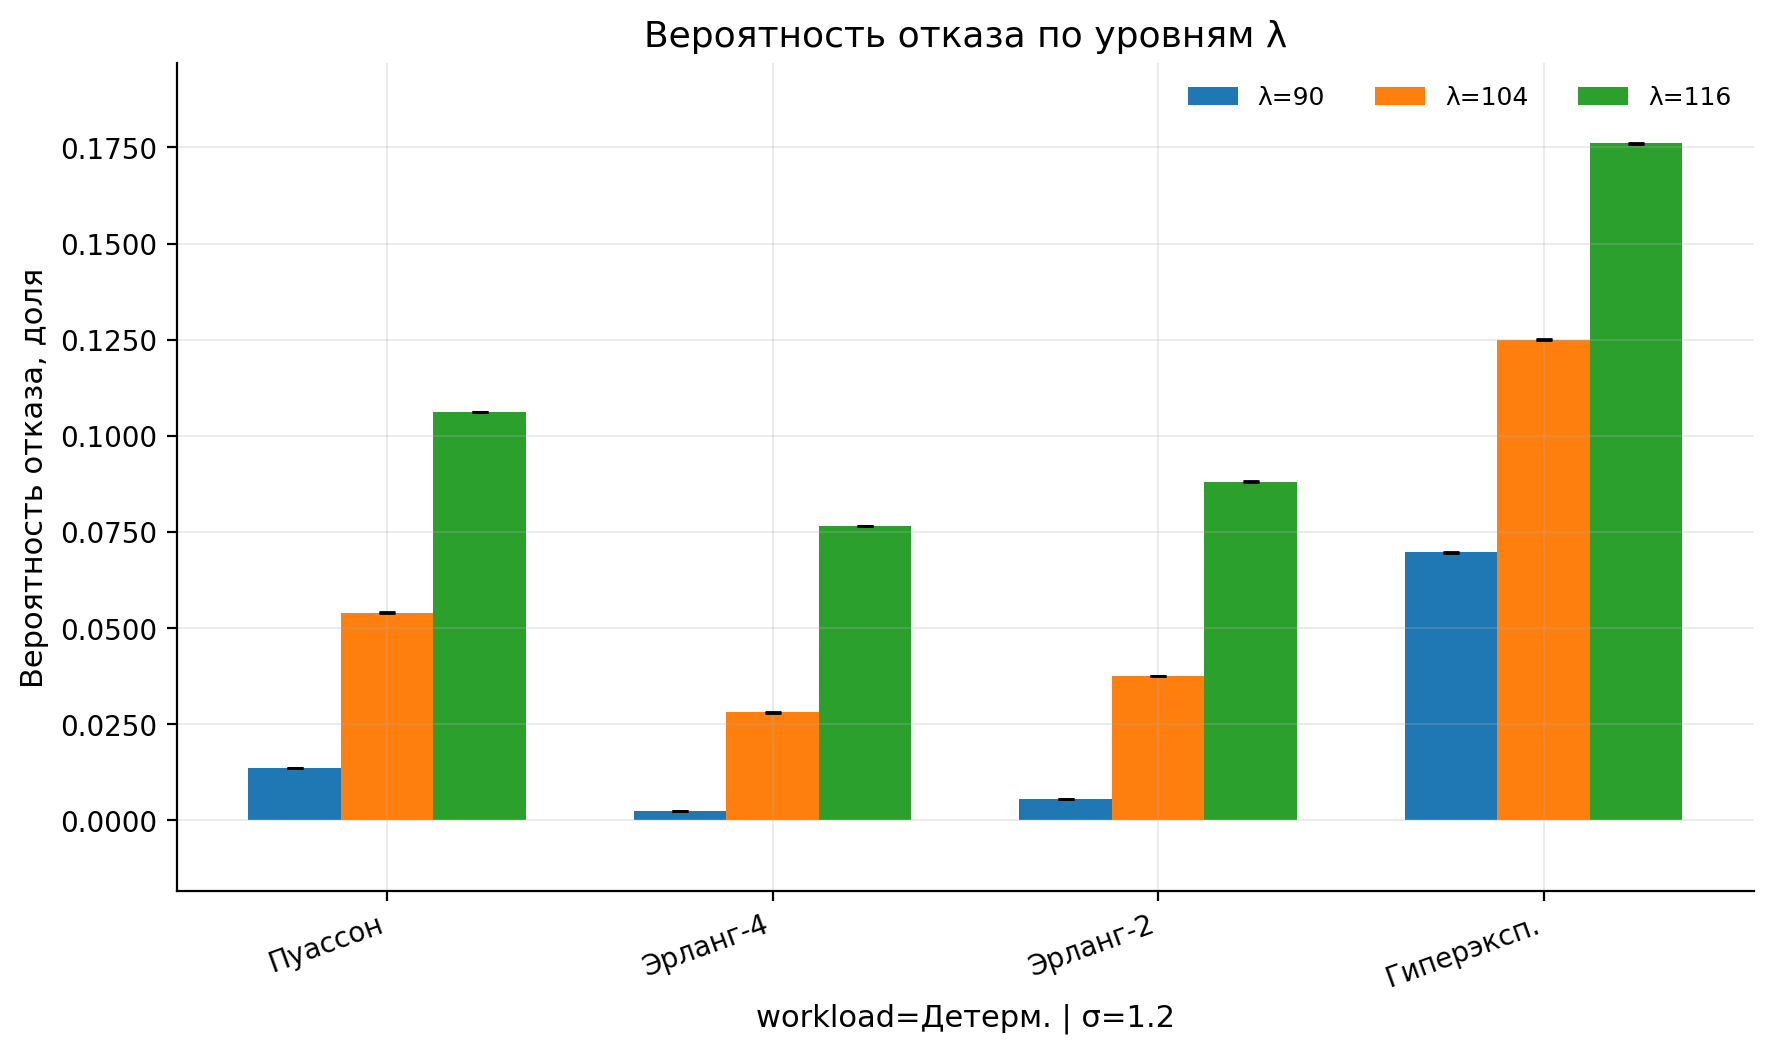
\includegraphics[
  width=\textwidth,
  height=0.55\textheight,
  keepaspectratio
]{arrival_sensitivity_loss_probability_bars_by_lambda_sigma-1p2.png}
\end{column}
\end{columns}

\vspace{0.1cm}
Регулярность (например Эрланг) снижает потери, а пачечность (Гиперэксп.) их резко увеличивает. 

Тип потока — более значемый фактор чувствительности.

\end{frame}

% ------------------------------------------------------------
% 9.2. Arrival: Механика состояний
% ------------------------------------------------------------
\begin{frame}{Изменение стационарного распределения $\pi(k)$}

\begin{columns}[T,totalwidth=\textwidth]
\begin{column}{0.46\textwidth}
\textbf{Динамика состояний системы:}
\begin{itemize}
  \item Кривые $\pi(k)$ строго разделяются (различия статистически значимы).
  \item \textbf{Эрланг:} загрузка смещена вправо, но равномерная.
  \item \textbf{HyperExp:} убывает медленно, система упирается в лимит по $R$.
\end{itemize}
\end{column}

\begin{column}{0.52\textwidth}
\centering
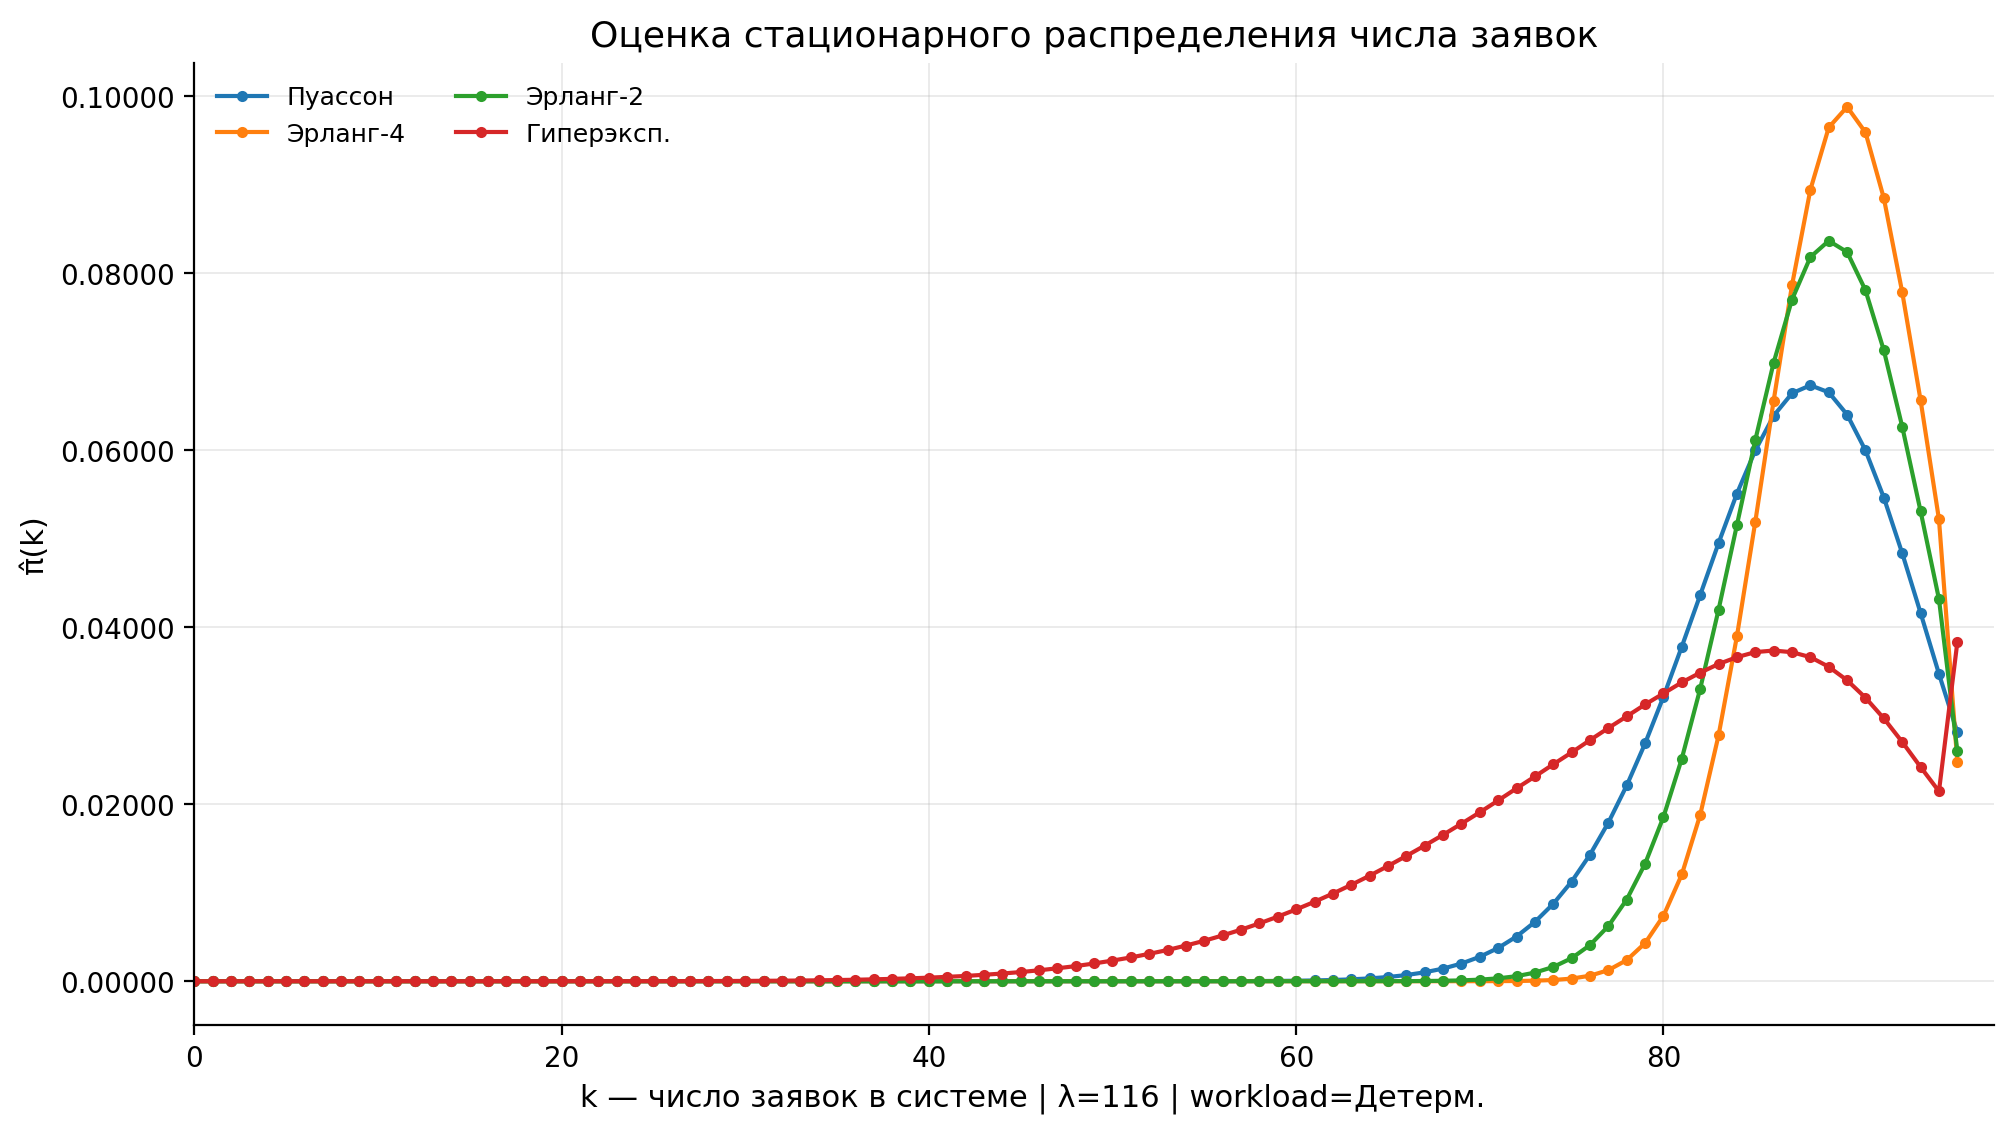
\includegraphics[
  width=\textwidth,
  height=0.55\textheight,
  keepaspectratio
]{arrival_sensitivity_stationary_distribution_sigma-1p2_lambda-116.png}
\end{column}
\end{columns}

\vspace{0.1cm}
Среднего значения $\lambda$ недостаточно для оценки потерь. Критически важна дисперсия потока $c_A^2$.

\end{frame}

% ------------------------------------------------------------
% 10. Совместное влияние: Тепловая карта
% ------------------------------------------------------------
\begin{frame}{Совместное влияние}

\begin{columns}[T,totalwidth=\textwidth]
\begin{column}{0.46\textwidth}
\textbf{Анализ матрицы сценариев:}
\begin{itemize}
  \item \textbf{Пуассоновский вход} (слева): $P_{\mathrm{loss}}$ идентичны — \textit{инвариантность сохраняется}.
  \item \textbf{Непуассоновские потоки}: инвариантность \textit{нарушается} (строки отличаются).
  \item Тип потока задаёт базу потерь, а workload лишь модулирует её.
\end{itemize}
\end{column}

\begin{column}{0.52\textwidth}
\centering
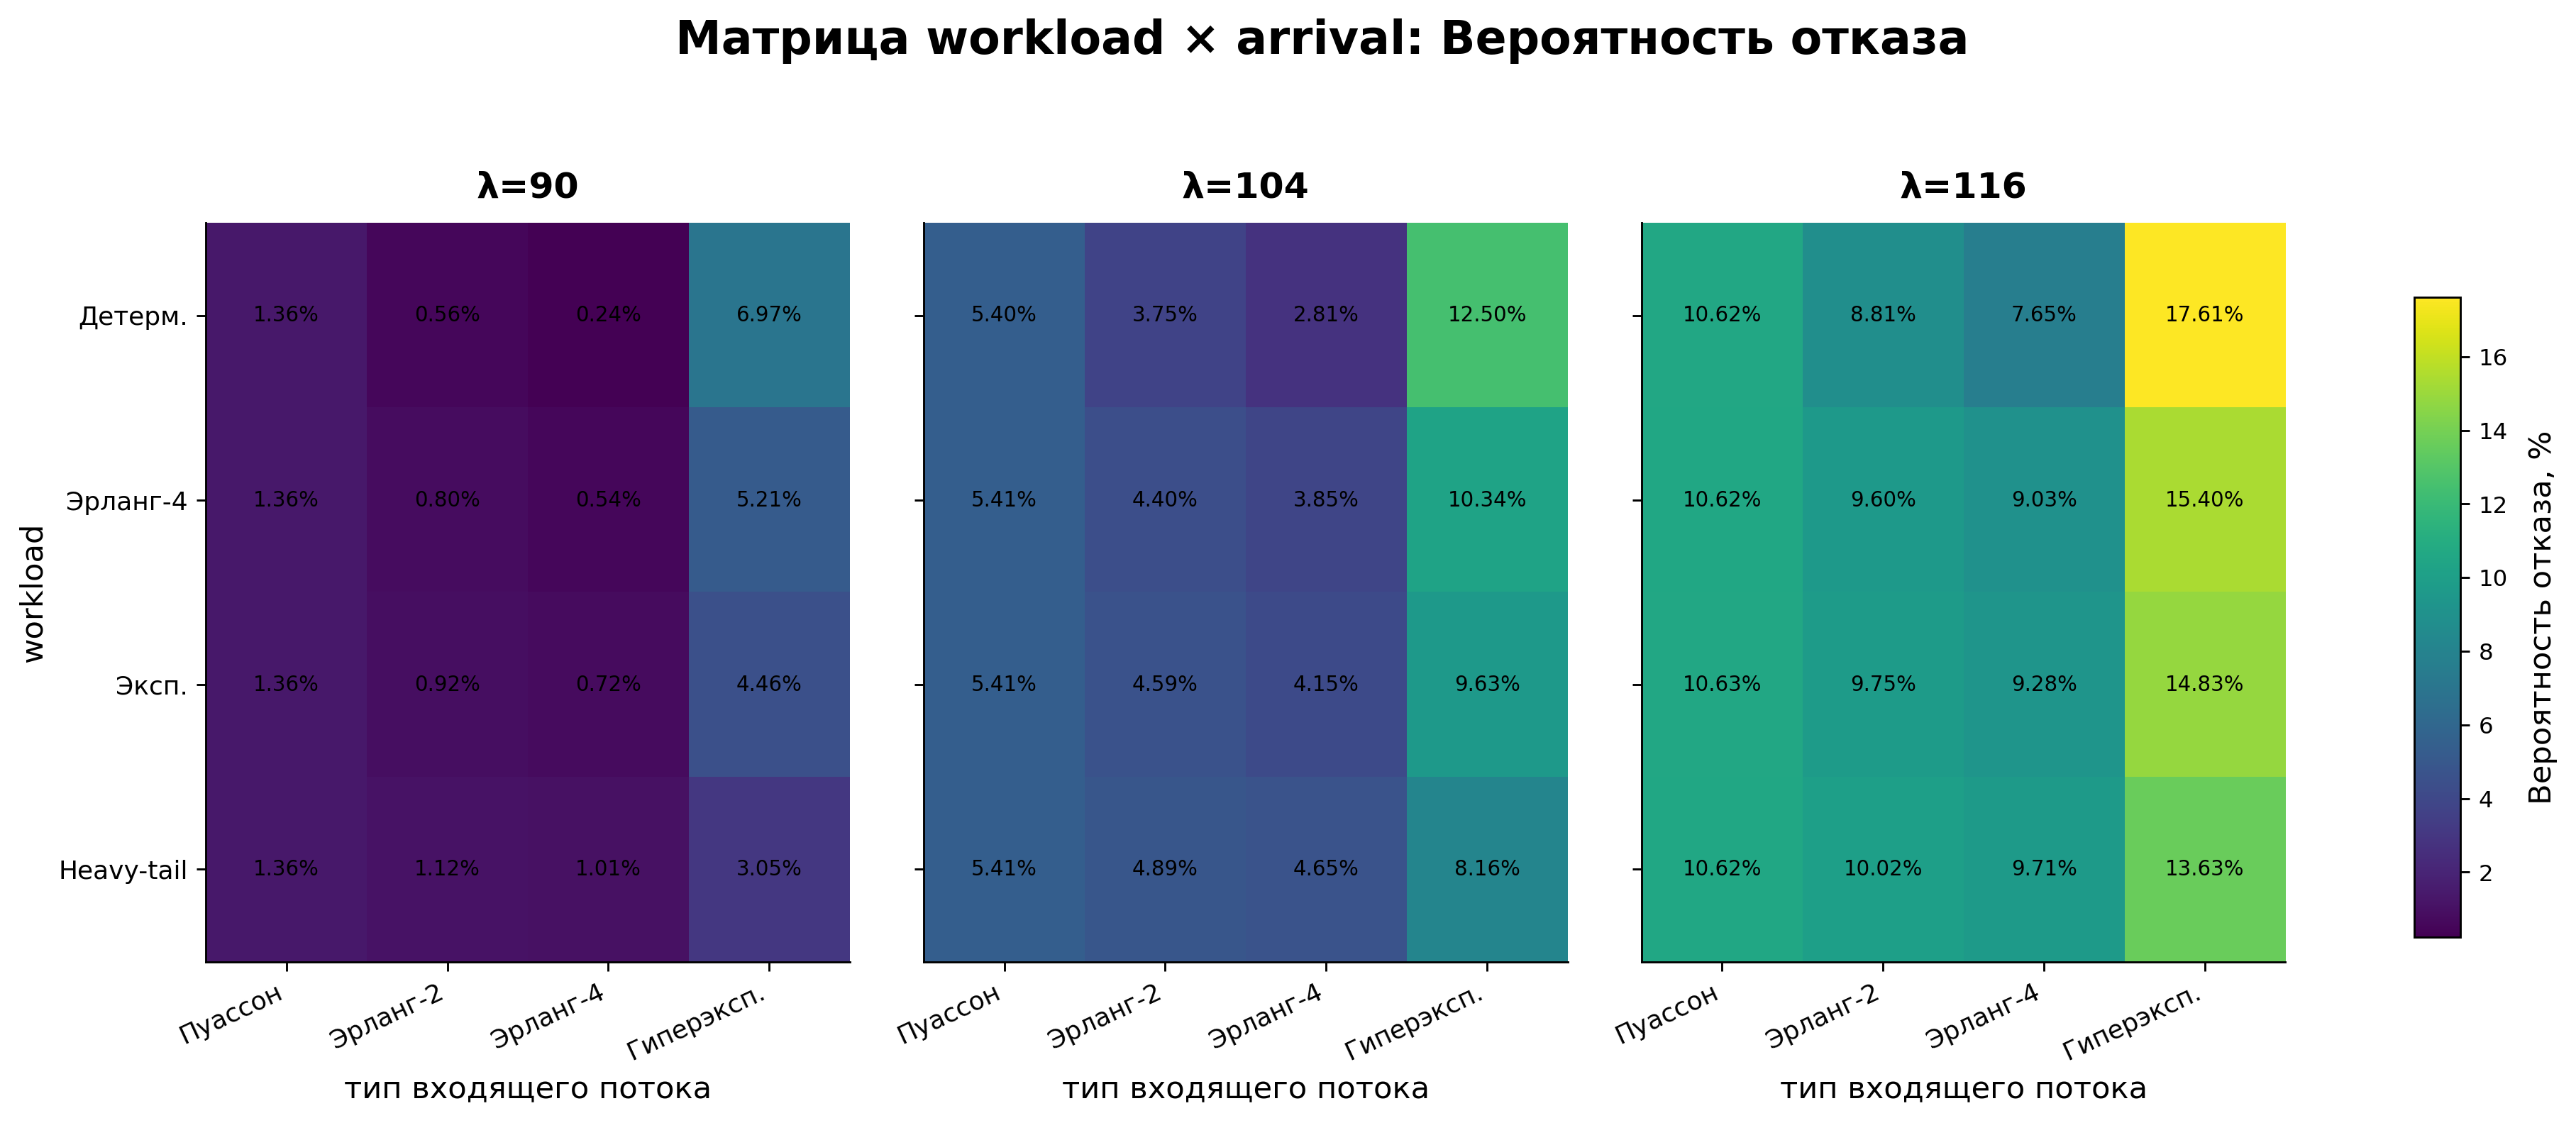
\includegraphics[
  width=\textwidth,
  height=0.42\textheight,
  keepaspectratio
]{01_heatmap_workload_arrival_loss_probability_sigma-1p2}
\end{column}
\end{columns}

\vspace{0.1cm}
Влияние обслуживания проявляется только во взаимодействии с характером входящего потока.

\end{frame}

% ------------------------------------------------------------
% 11. Взаимодействие факторов (Дельта)
% ------------------------------------------------------------
\begin{frame}{Взаимодействие потока и обслуживания}

\begin{columns}[T,totalwidth=\textwidth]
\begin{column}{0.46\textwidth}
\begin{itemize}
  \item \textbf{Регулярный вход} дает минимум потерь при константном обслуживании.
  \item \textbf{Пачечный вход} "забивает" систему при стабильном обслуживании. Высоковариативное обслуживание "разбивает" пачки и снижает потери.
\end{itemize}
\end{column}

\begin{column}{0.52\textwidth}
\centering
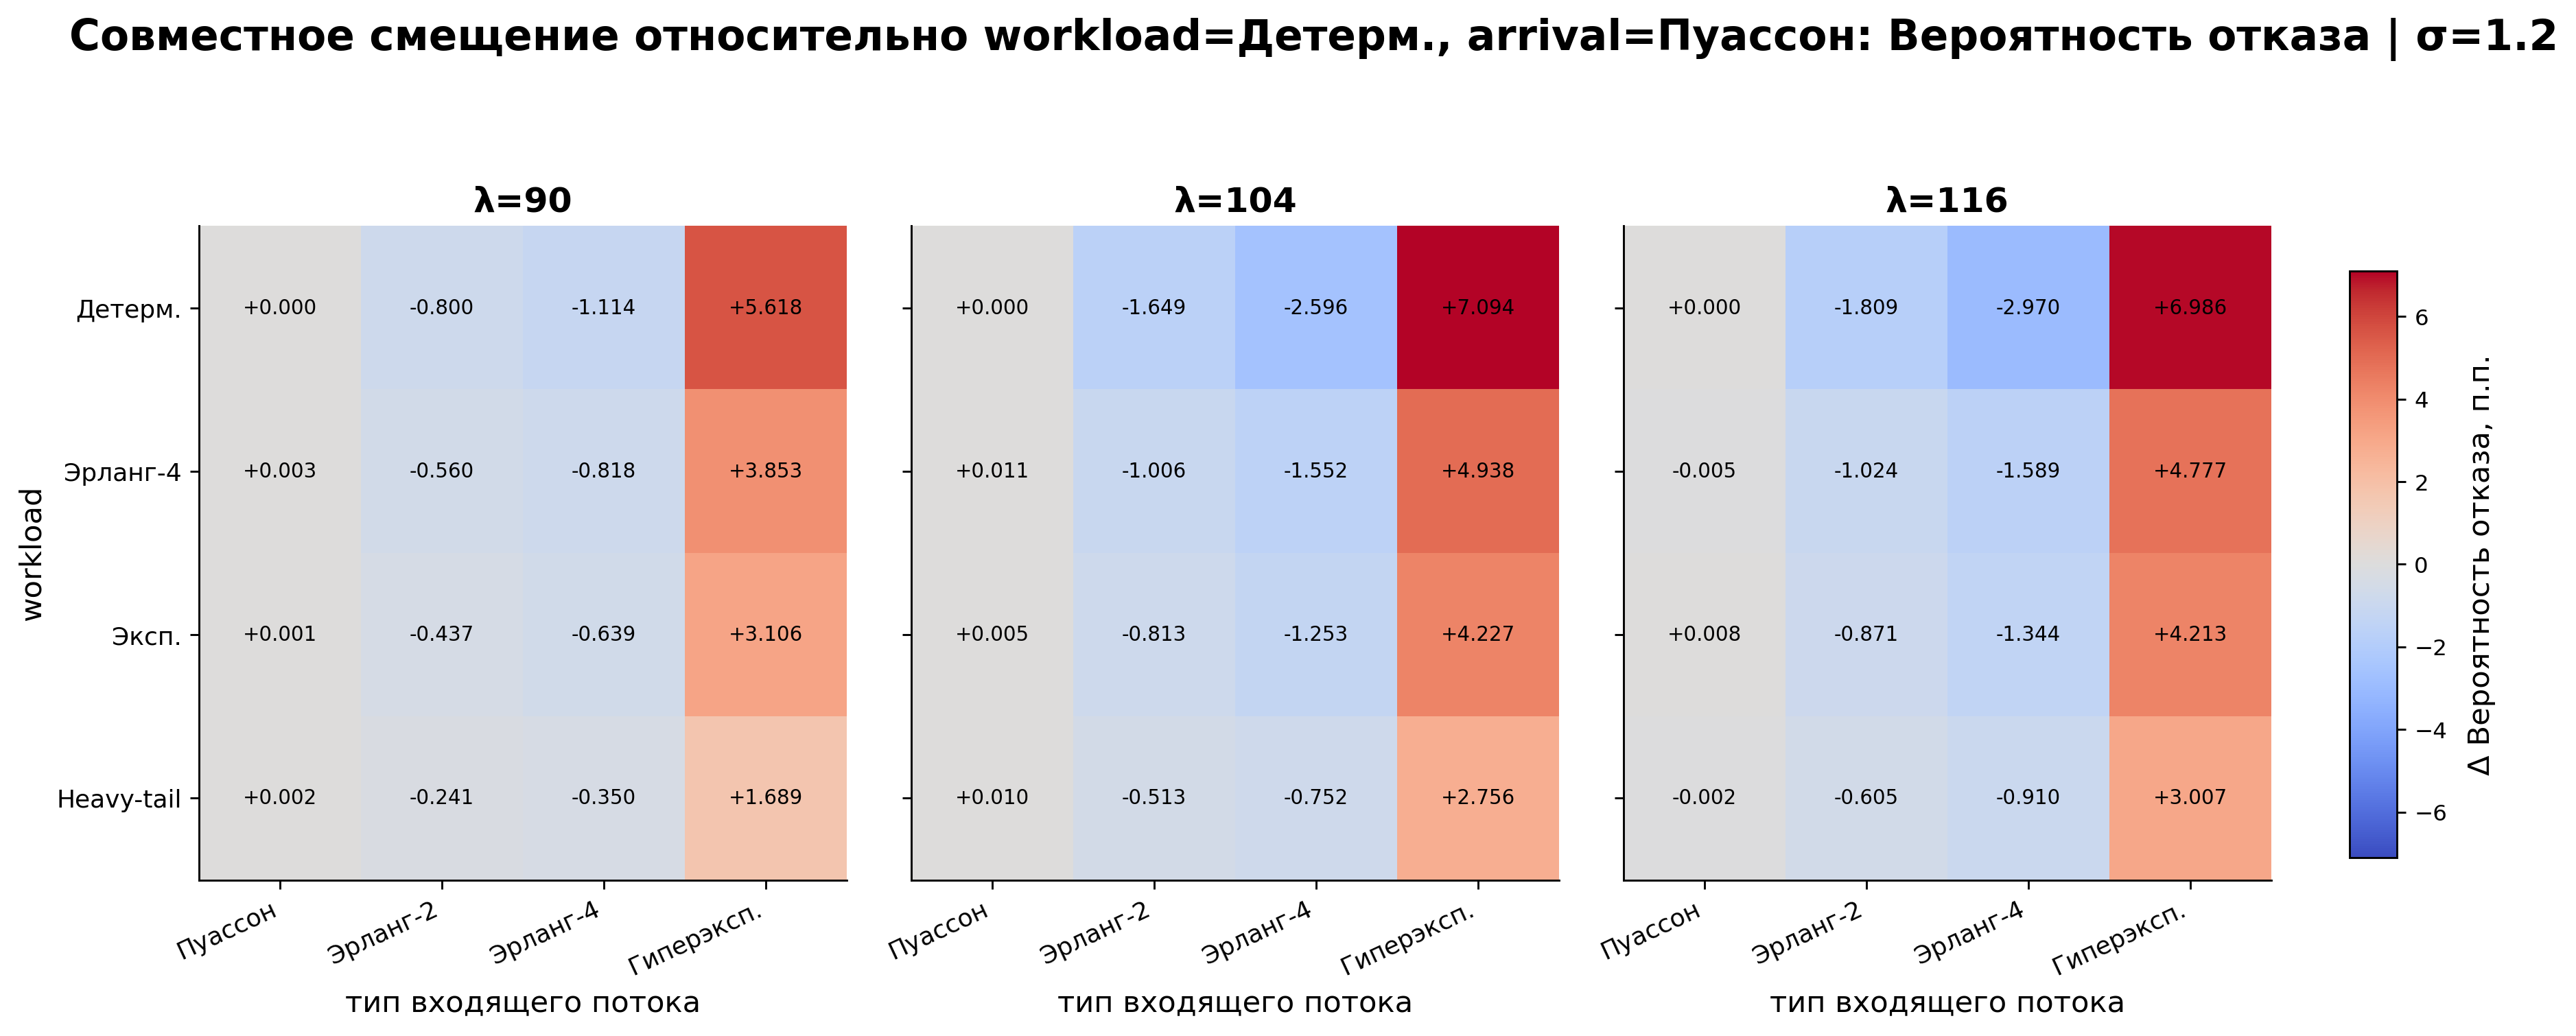
\includegraphics[
  width=\textwidth,
  height=0.42\textheight,
  keepaspectratio
]{06_joint_delta_vs_det_poisson_loss_probability_sigma-1p2}
\end{column}
\end{columns}

\vspace{0.1cm}
Знак производной $\frac{\partial P_{\mathrm{loss}}}{\partial c_B^2}$ меняется в зависимости от дисперсии входящего потока $c_A^2$.

\end{frame}

% ------------------------------------------------------------
% 12.1. Структура отказов (График)
% ------------------------------------------------------------
\begin{frame}{Декомпозиция структуры отказов}

\begin{center}
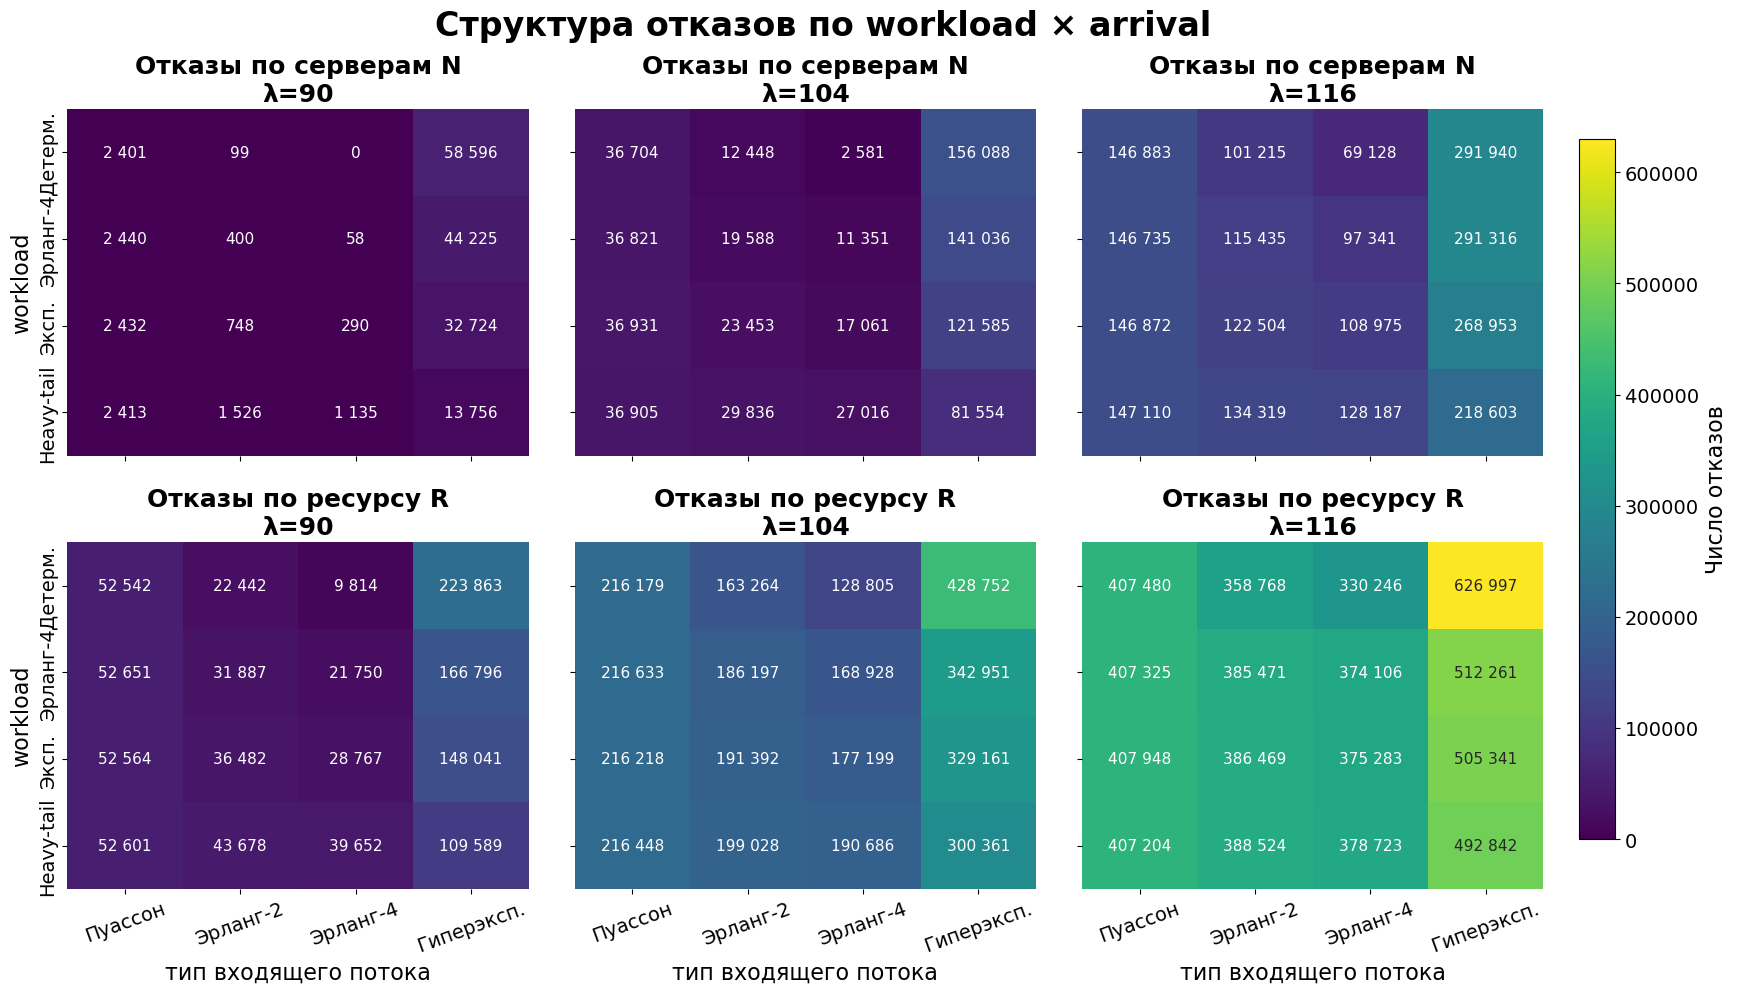
\includegraphics[
  width=\textwidth,
  height=0.82\textheight,
  keepaspectratio
]{08_rejection_components_heatmaps_sigma-1p2_2}
\end{center}

\end{frame}

% ------------------------------------------------------------
% 12.2. Структура отказов и совместное влияние
% ------------------------------------------------------------
\begin{frame}{Влияние распределений на структуру отказов}

Абсолютное большинство заявок теряется из-за исчерпания ресурса ($R$). Отказы по нехватке серверов ($N$) минимальны во всех сценариях.

\vspace{0.2cm}
Для всех уровней нагрузки строго сохраняется математический порядок вероятности отказа:
$$ P_{\mathrm{loss}}(\text{Erlang-4}) < P_{\mathrm{loss}}(\text{Erlang-2}) < P_{\mathrm{loss}}(\text{Poisson}) < P_{\mathrm{loss}}(\text{HyperExp}) $$

\vspace{0.1cm}
\begin{itemize}
  \item \textbf{Лучший сценарий:} регулярный вход (Erlang-4) + детерминированное обслуживание.
  \item \textbf{Худший сценарий:} пачечный вход (HyperExp) + детерминированное обслуживание.
  \item \textbf{Эффект сглаживания:} негативное влияние пачечного трафика компенсируется высоковариативным обслуживанием.
\end{itemize}

\end{frame}

% ------------------------------------------------------------
% 13. Общее заключение
% ------------------------------------------------------------
\begin{frame}{Основные результаты и выводы}

\begin{enumerate}
  \item Формализована ресурсная модель $GI/G/N/N/R$. Разработан симулятор, эффективно выполняющий независимые репликации Монте-Карло.
  \item Эмпирически подтверждено, что при пуассоновском входе макропоказатели системы строго инвариантны к форме распределения времени обслуживания.
  \item Установлено, что регулярные входящие потоки минимизируют отказы, а пачечные — кратно их увеличивают.
  \item При немарковском входе инвариантность нарушается. Влияние формы обслуживания строго зависит от дисперсии входящего потока.
\end{enumerate}

\vspace{0.1cm}
Для оценки чувствительности в первую очередь необходимо учитывать среднюю нагрузку $\lambda$, затем форму входящего потока, и наконец — её взаимодействие с обслуживанием.

\end{frame}

% ------------------------------------------------------------
% 14. Thanks
% ------------------------------------------------------------
\begin{frame}{Спасибо за внимание}

\vspace{1.7cm}

\begin{center}
{\Huge\color{rudnblue}\bfseries Спасибо за внимание!}

\vspace{0.9cm}

{\Large Готов ответить на ваши вопросы.}
\end{center}

\end{frame}

\end{document}